\documentclass{beamer}
\usepackage{../tut-slides}
\usepackage{../mathoperatorsAuD}

\usepackage{lmodern}
\usepackage{csquotes}
\usepackage{amsmath,amssymb}
\usepackage{stmaryrd}
\usepackage{enumerate}
%\usepackage[inline]{enumitem} 		%customize label
%\newcommand{\labelitemi}{\raisebox{1pt}{\scalebox{.9}{$\blacktriangleright$}}}
%\newcommand{\labelitemii}{$\vartriangleright$}
%\newcommand{\labelitemiii}{--}
\setbeamertemplate{itemize item}{\raisebox{1pt}{\scalebox{.9}{$\blacktriangleright$}}}
\setbeamertemplate{itemize subitem}{$\vartriangleright$}

\usepackage{booktabs}
\usepackage{tabularx}
\usepackage{tabu}
\newcommand*\head{\rowfont{\bfseries}}
\newcommand*{\tw}{\rowfont{\ttfamily}}
\renewcommand{\tabularxcolumn}[1]{>{\hspace{0pt}}m{#1}}
\usepackage{multirow}

\usepackage{cancel}

\usepackage{empheq}
\newcommand*\widefbox[1]{\fbox{\hspace{2em} #1 \hspace{2em}}}

\usepackage[many]{tcolorbox}
\tcbuselibrary{listings}
\newtcolorbox{mymathbox}[1][]{colback=white, sharp corners, #1}

\usepackage{xcolor}
\usepackage{listings}
\usepackage{bold-extra}
\newcommand*{\ttfamilywithbold}{\fontfamily{lmtt}\selectfont}

\lstset{numbers=left, 
	numberstyle=\tiny, 
	breaklines=true,
%	backgroundcolor=false,
	numbersep=5pt,
	language=C,
	tabsize=2,
	basicstyle=\footnotesize\ttfamily,
	showstringspaces=false,
	frame=tb} 

\lstdefinestyle{notebook}{
	basicstyle=\footnotesize\ttfamilywithbold,   
	breakatwhitespace=false,         
	breaklines=true,                 
	commentstyle=\itshape, 
	escapeinside={\%*}{*)},          % if you want to add LaTeX within your code
	extendedchars=true,              % lets you use non-ASCII characters; for 8-bits encodings only, does not work with UTF-8
	backgroundcolor=\color{cdgray!10},
	frame=single,
	keywordstyle=\bfseries,       % keyword style
	morekeywords={}, 
	language=C,                 % the language of the code
	numbers=left,                    % where to put the line-numbers; possible: (none, left, right)
	numbersep=5pt,                   
	numberstyle=\tiny\color{cdgray!50}, 
	rulecolor=\color{cddarkblue}, 
	tabsize=2,
	frameround=tttt
}

\DeclareMathOperator{\ack}{\mathbf{ack}}
\usepackage{MnSymbol}

\newcommand{\col}[1]{\textcolor{cdpurple}{#1}}
\newcolumntype{R}[1]{>{\centering\arraybackslash}p{#1}}

%%%% EBNF-Terme %%%%
\newcommand{\wdh}[1]{\hat{\{} \ #1 \ \hat{\}}}
\newcommand{\opt}[2]{\hat{(} \ #1 \ \hat{|} \ #2 \ \hat{)}}
\newcommand{\byp}[1]{\hat{[} \ #1 \ \hat{]}}
\newcommand{\rdb}[1]{\hat{(} \ #1 \ \hat{)}}

\begin{document}	
	\title{Algorithmen und Datenstrukturen}
	\subtitle{Übung 6: Arrays \& Listen}
	\author{Eric Kunze}
	\email{eric.kunze@mailbox.tu-dresden.de}
	\city{TU Dresden}
%	\institute{Lehrstuhl für Grundlagen der Programmierung}
	\titlegraphic{
\includegraphics[width=2cm]{../TUD-white.pdf}}
	\date{04.12.2020}

	\maketitle


%%%%%%%%%%%%%%%%%%%%%%%%%%%%%%%%%%%%%%%%%%%%%%%%%%%%%%%%%%%%%%%%%%%%%%%%%%%%%

\section{Arrays}

\begin{frame} \frametitle{Arrays}
	\begin{description}
		\item[Deklaration (als EBNF):]
		$\texttt{ElementType} \enskip \texttt{Ident} \enskip \wdh{\texttt{[} \texttt{Number} \texttt{]}}\enskip  \texttt{;}$ \vspace{-\baselineskip}
		\pause
		\begin{itemize}
			\item \texttt{ElementType} $\dots$ Typ eines Eintrags
			\item \texttt{Number} $\dots$ Anzahl der Einträge
			\item \texttt{Ident} $\dots$ Bezeichner des Arrays
		\end{itemize}
		\pause
		\item[Beispiele:]
		\begin{itemize}
			\item Liste: \lstinline{int liste[5];}
			\item Matrix: \lstinline{int matrix[3][4];}
		\end{itemize}
		\pause
		\item[Initialisierungen:] ~
		\begin{itemize}
			\item \lstinline|int liste[5] = \{2,7,0,-4,1\};|
			\item \lstinline{int matrix[3][4] = \{ \{1,2,3,4\}, \{5,6,7,8\}, \{2,3,4,5\} \};}
		\end{itemize}
		\pause
		\item[Zuweisungen:] \textit{Indizierung beginnt bei \texttt{0}}
		\begin{itemize}
			\item \lstinline{liste[2] = 16;} $\leadsto$ \lstinline{[2,7,16,-4,1]} 
			\item \lstinline{matrix[1][3] = 0;} $\leadsto$ $\left( \begin{smallmatrix} 1 & 2 & 3 & 4 \\ 5 & 6 & 7 & 0 \\ 2 & 3 & 4 & 5 \end{smallmatrix} \right)$
		\end{itemize}
	\end{description}
\end{frame}

\begin{frame}[fragile] \frametitle{Aufgabe 1}
	
	Ist die Zeichenkette ein Palindrom, so soll der aktuelle Parameter \texttt{korrekt} im Aufruf von \texttt{palindrom1}
	den Wert \texttt{1} annehmen, sonst \texttt{0}.
	
	\textbf{falscher Code:}
	\begin{lstlisting}
		palindrom1(char feld[], int l, int korrekt) {
			int i = 1;
			l = l - 1;
			while (i < l && korrekt) {
				korrekt = feld[i] == feld[l];
				i = i + 1;
			}
			return korrekt;
		}
	\end{lstlisting}
\end{frame}

\begin{frame}[fragile] \frametitle{Aufgabe 1}
	\textbf{richtiger Code:} \pause
	\begin{lstlisting}[style=notebook]
		void palindrom1(char feld[], int l, int *korrekt) {
			int i = 0;    // muss mit 0 statt 1 initialisiert werden
			l = l - 1;
			*korrekt = 1; // muss mit 1 initialisiert werden
			while (i < l && *korrekt) {
				*korrekt = feld[i] == feld[l];
				i = i + 1;
				l = l - 1;  // l muss dekrementiert werden
			}
			// kein return, weil rueckgabetyp void
		}
	\end{lstlisting}
\end{frame}

\section{Verkettete Listen}

\begin{frame}[fragile] \frametitle{Verkettete Listen}
	Wir betrachten \textit{verkettete} Listen.
	\begin{itemize}
		\item Listenelemente
		\item Verkettungen
	\end{itemize}
	
	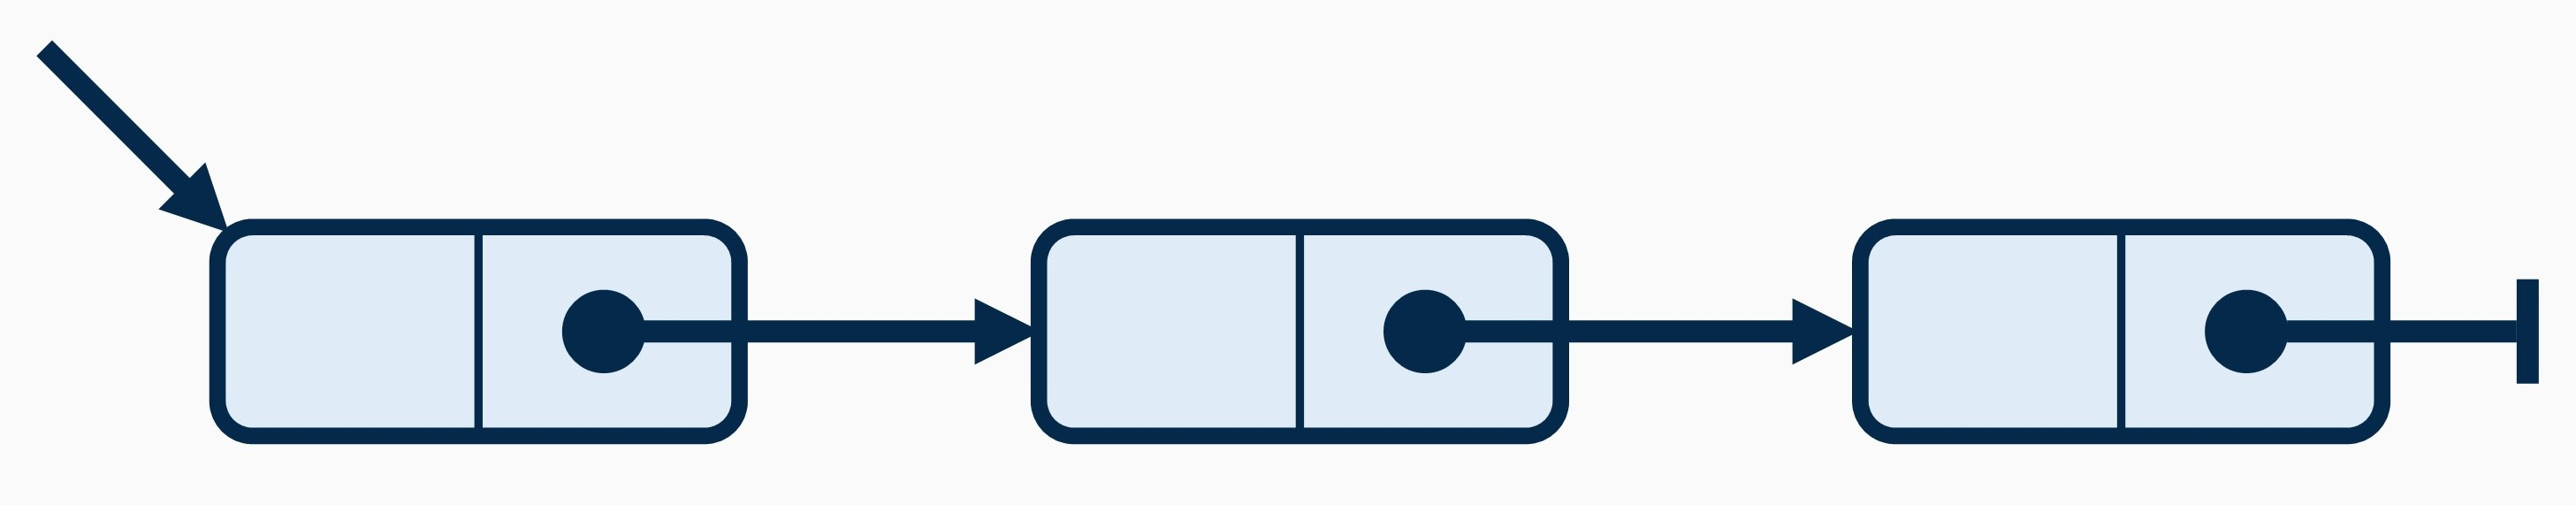
\includegraphics[width=\linewidth]{tut06-graphics/tut06-liste.jpg}
\end{frame}
\begin{frame}[fragile] \frametitle{Verkettete Listen}
	\footnotesize
	\begin{lstlisting}[style=notebook]
typedef struct element *list;
struct element {int value; list next};
	\end{lstlisting}
	\begin{itemize}
		\item \lstinline{struct element} definiert einen neuen Datentypen
		\item \lstinline{int value} ist der Wert des Listenelements
		\item \texttt{typedef} definiert nur einen Alias
		\begin{itemize} \scriptsize
			\item Wir dürfen jeden Pointer auf ein \lstinline{struct element} auch einfach \lstinline{list} nennen.
		\end{itemize}
		\item \lstinline{list next} ist ein Element vom Typ \lstinline{list}
		\begin{itemize} \scriptsize
			\item ein Pointer auf ein \lstinline{struct element} (das nächste Listenelement)
		\end{itemize}
	\end{itemize}
	\begin{center}
		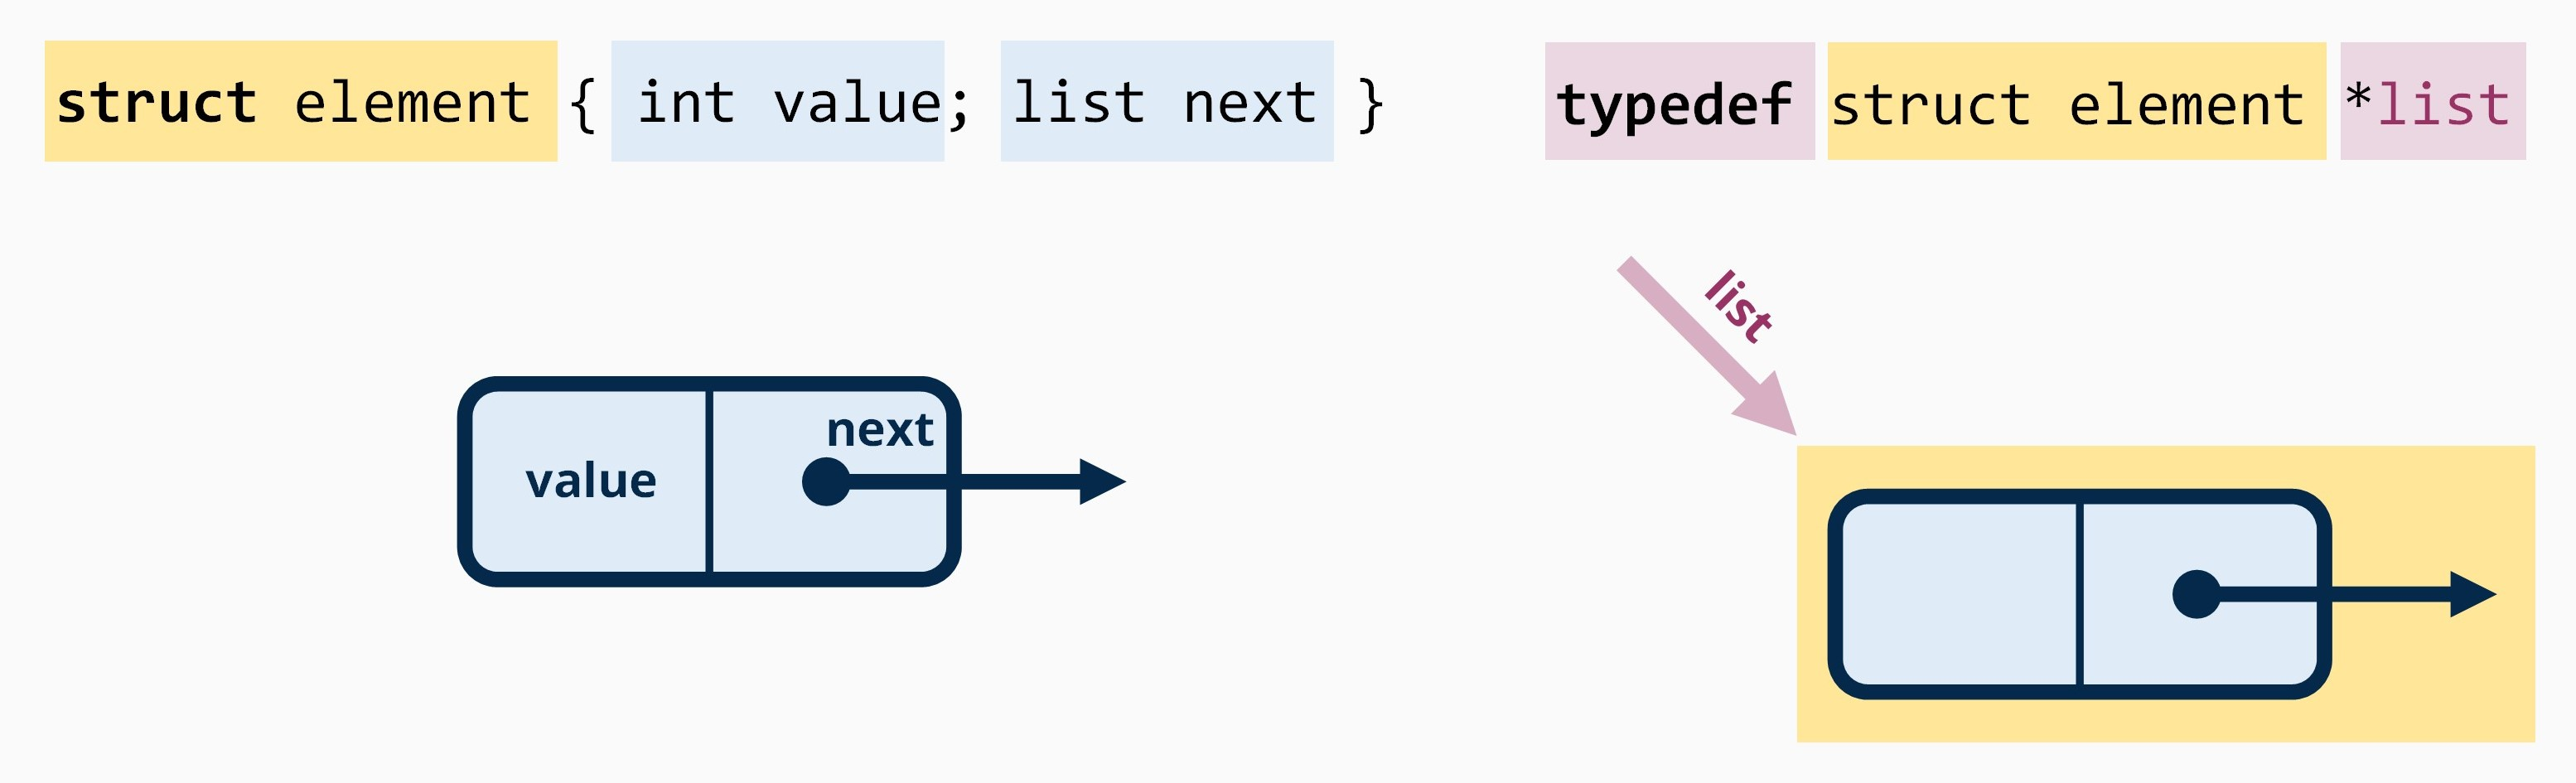
\includegraphics[width=.8\linewidth]{tut06-graphics/tut06-liste-impl}
	\end{center}
\end{frame}

\begin{frame}[fragile] \frametitle{Die Operatoren \texttt{\&}, \texttt{*}, \texttt{->}, \texttt{.}}
	\begin{center}
		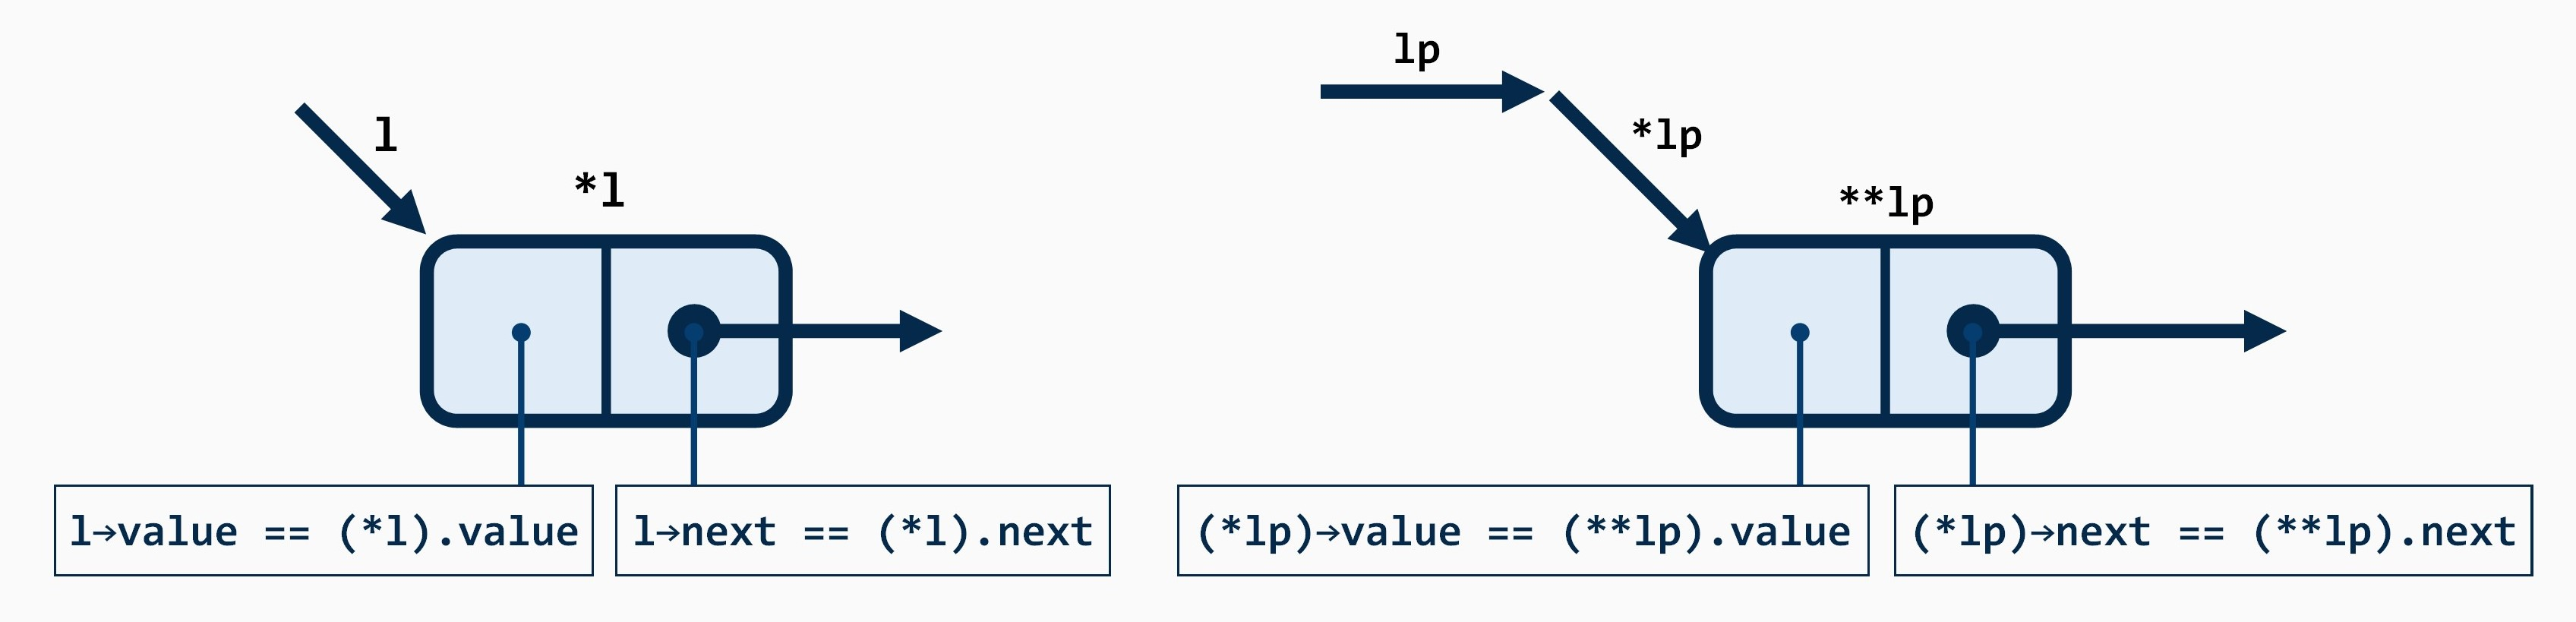
\includegraphics[width=\linewidth]{tut06-graphics/tut06-liste-zugriff}
	\end{center}

	Die Operatoren \texttt{\&} und \texttt{*} binden schwächer als \texttt{.} und \texttt{->}.
	\begin{itemize}
		\item \lstinline{l->value == (*l).value}
		\item \lstinline{&l->next == &((*l).next)}
	\end{itemize}
\end{frame}

\begin{frame} \frametitle{Aufgabe 2 --- Teil (a)}
	\textbf{Anfügen an eine Liste}
	
	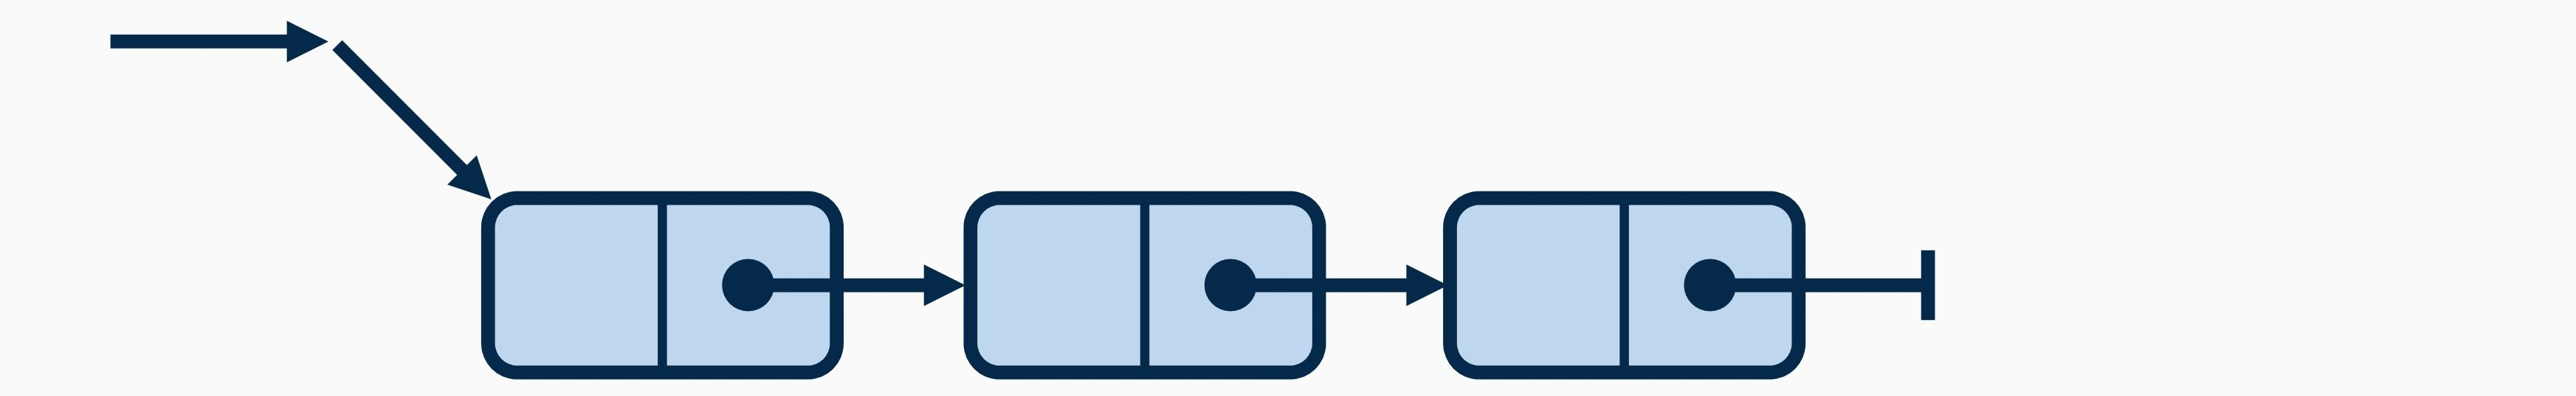
\includegraphics[width=\linewidth]{tut06-graphics/tut06-append1} \\ \pause
	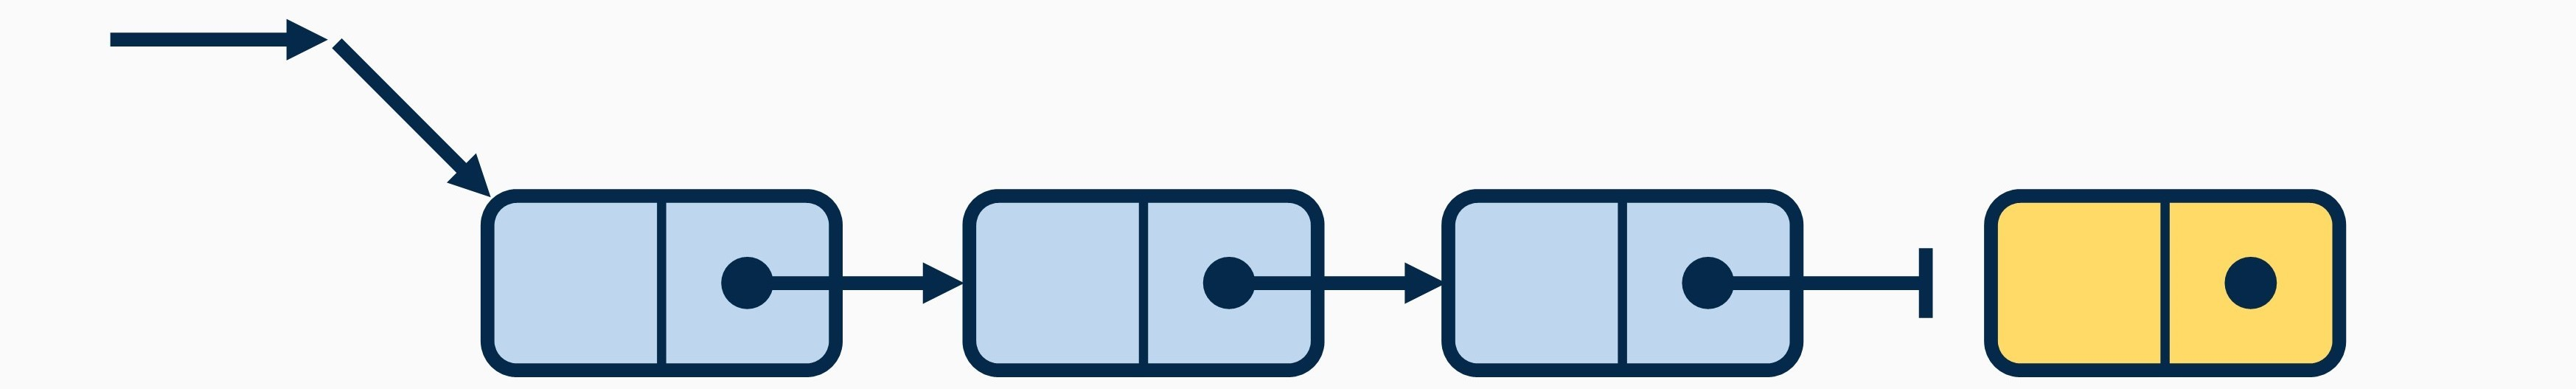
\includegraphics[width=\linewidth]{tut06-graphics/tut06-append2} \\ \pause
	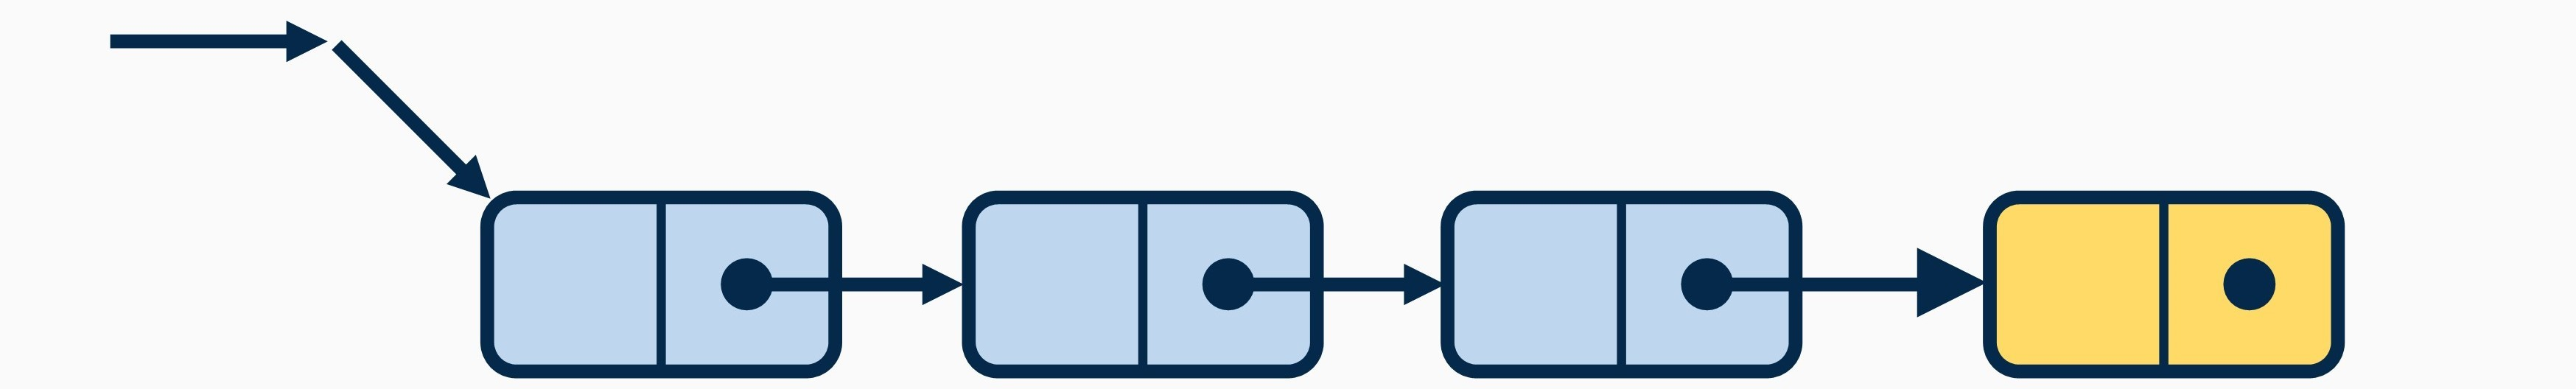
\includegraphics[width=\linewidth]{tut06-graphics/tut06-append3} \\ \pause
	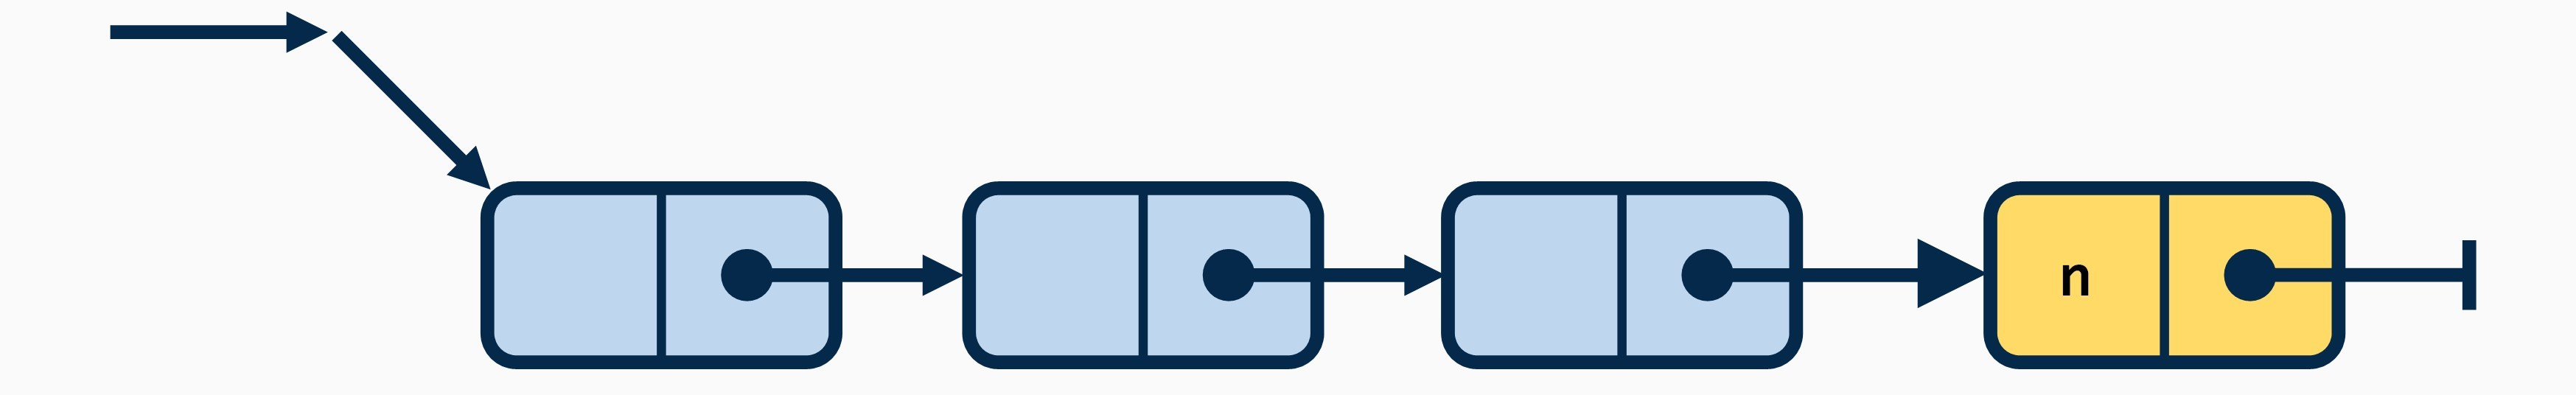
\includegraphics[width=\linewidth]{tut06-graphics/tut06-append4}
\end{frame}

\begin{frame}[fragile] \frametitle{Aufgabe 2 --- Teil (a)}
	\textbf{Anfügen an eine Liste}
	
	\begin{center}
		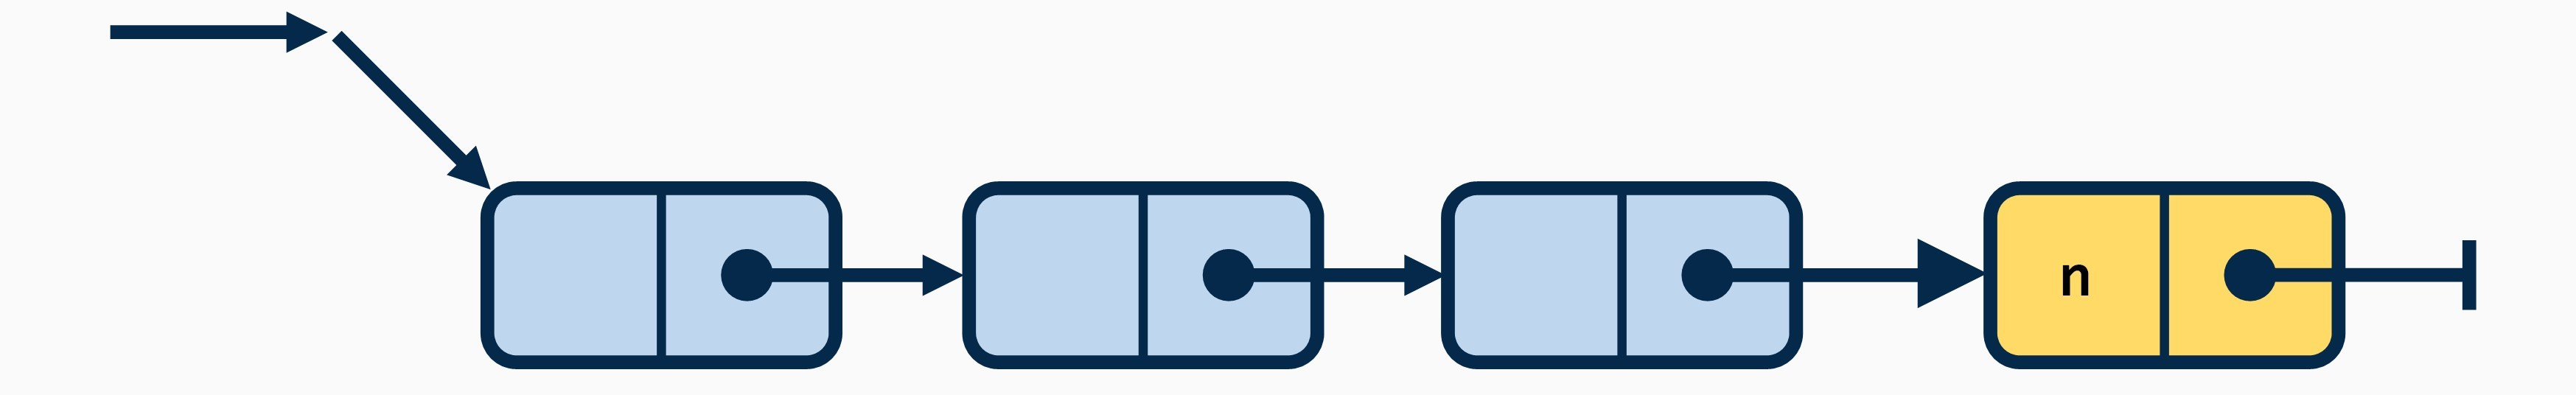
\includegraphics[width=\linewidth]{tut06-graphics/tut06-append4}
	\end{center}

	\pause
	
	\begin{itemize}
		\item Gehe zum Ende der Liste
		\item Allokiere neuen Speicherplatz und verknüpfe mit neues Element mit bisheriger Liste
		\begin{itemize}
			\item Nachfolger-Pointer des bisherigen letzen Listenelements auf auf neues Listenelement zeigen lassen
		\end{itemize}
		\item Fülle das Listenelement mit Schlüsselwert und Nachfolger (= \texttt{NULL})
	\end{itemize}
\end{frame}

\begin{frame}[fragile] \frametitle{Aufgabe 2 --- Teil (a)}
	\textbf{Anfügen an eine Liste}
	\begin{itemize}
		\item Gehe zum Ende der Liste
		\item Allokiere neuen Speicherplatz und verknüpfe mit neues Element mit bisheriger Liste
		\begin{itemize}
			\item Nachfolger-Pointer des bisherigen letzen Listenelements auf auf neues Listenelement zeigen lassen
		\end{itemize}
		\item Fülle das Listenelement mit Schlüsselwert und Nachfolger (= \texttt{NULL})
	\end{itemize}

	\pause
	
	\begin{lstlisting}[style=notebook]
	void append(list *lp, int n){
			while(*lp != NULL) 
					lp = &((*lp)->next) ; 
			(*lp) = malloc(sizeof(struct element)); 
			(*lp)->key  = n;   
			(*lp)->next = NULL; 
	}
	\end{lstlisting}
\end{frame}

\begin{frame}[fragile] \frametitle{Aufgabe 2 --- Teil (b)}
	\textbf{Liste erstellen (mit \texttt{append})}
	\begin{itemize}
		\item erzeuge leere Liste
		\item hänge Listenelemente an leere Liste an (durch Aufrufe von \texttt{append})
	\end{itemize}
	
	\pause
	
	\begin{lstlisting}[style=notebook]
	list l = NULL;
	append(&l, 4);
	append(&l, 2);
	append(&l, 0);
	\end{lstlisting}
\end{frame}

\begin{frame}[fragile] \frametitle{Aufgabe 2 --- Teil (c)}
	\textbf{Summe einer Liste --- iterativ}
	\begin{itemize} \small
		\item addiere Schlüsselwerte in Hilfsvariable \texttt{result} auf
		\item laufe Liste entlang  $\to$ Pointer immer weiter \enquote{schalten}
	\end{itemize}

	\pause

	\begin{center}
		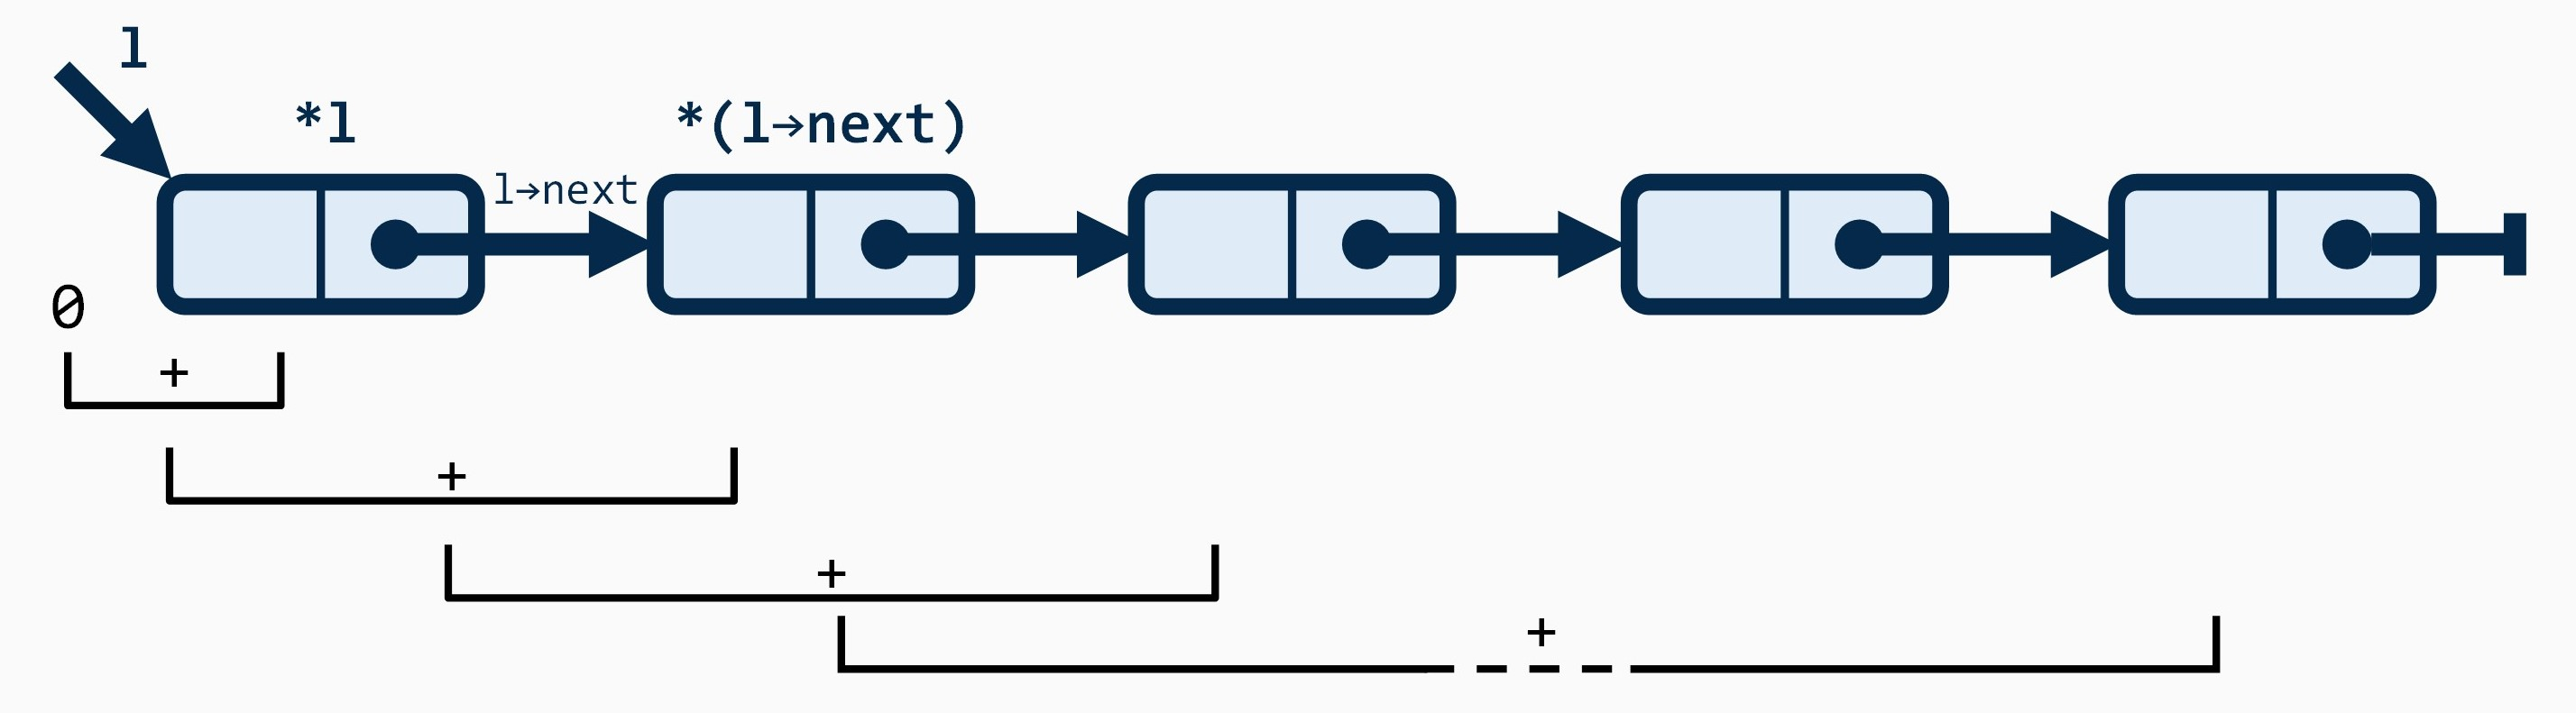
\includegraphics[width=0.7\linewidth]{tut06-graphics/tut06-summe-it}
	\end{center}

	\pause
	
	\begin{lstlisting}[style=notebook, basicstyle=\scriptsize\ttfamilywithbold]
	int sum_it(list l) {
		int result = 0;
		while (l != NULL) {
			result = result + l->value;
			l = l->next;   // "start"zeiger weiterschalten 
		}
		return result;
	}
	\end{lstlisting}
\end{frame}

\begin{frame}[fragile] \frametitle{Aufgabe 2 --- Teil (c)}
	\textbf{Summe einer Liste --- rekursiv}
	\begin{itemize}
		\item definiere Basisfall: leere Liste $\to$ Rückgabewert \texttt{0}
		\item rufe Funktion rekursiv auf --- mit \texttt{next}-Pointer als neuen Startpointer
	\end{itemize}

	\pause
	
	\begin{center}
		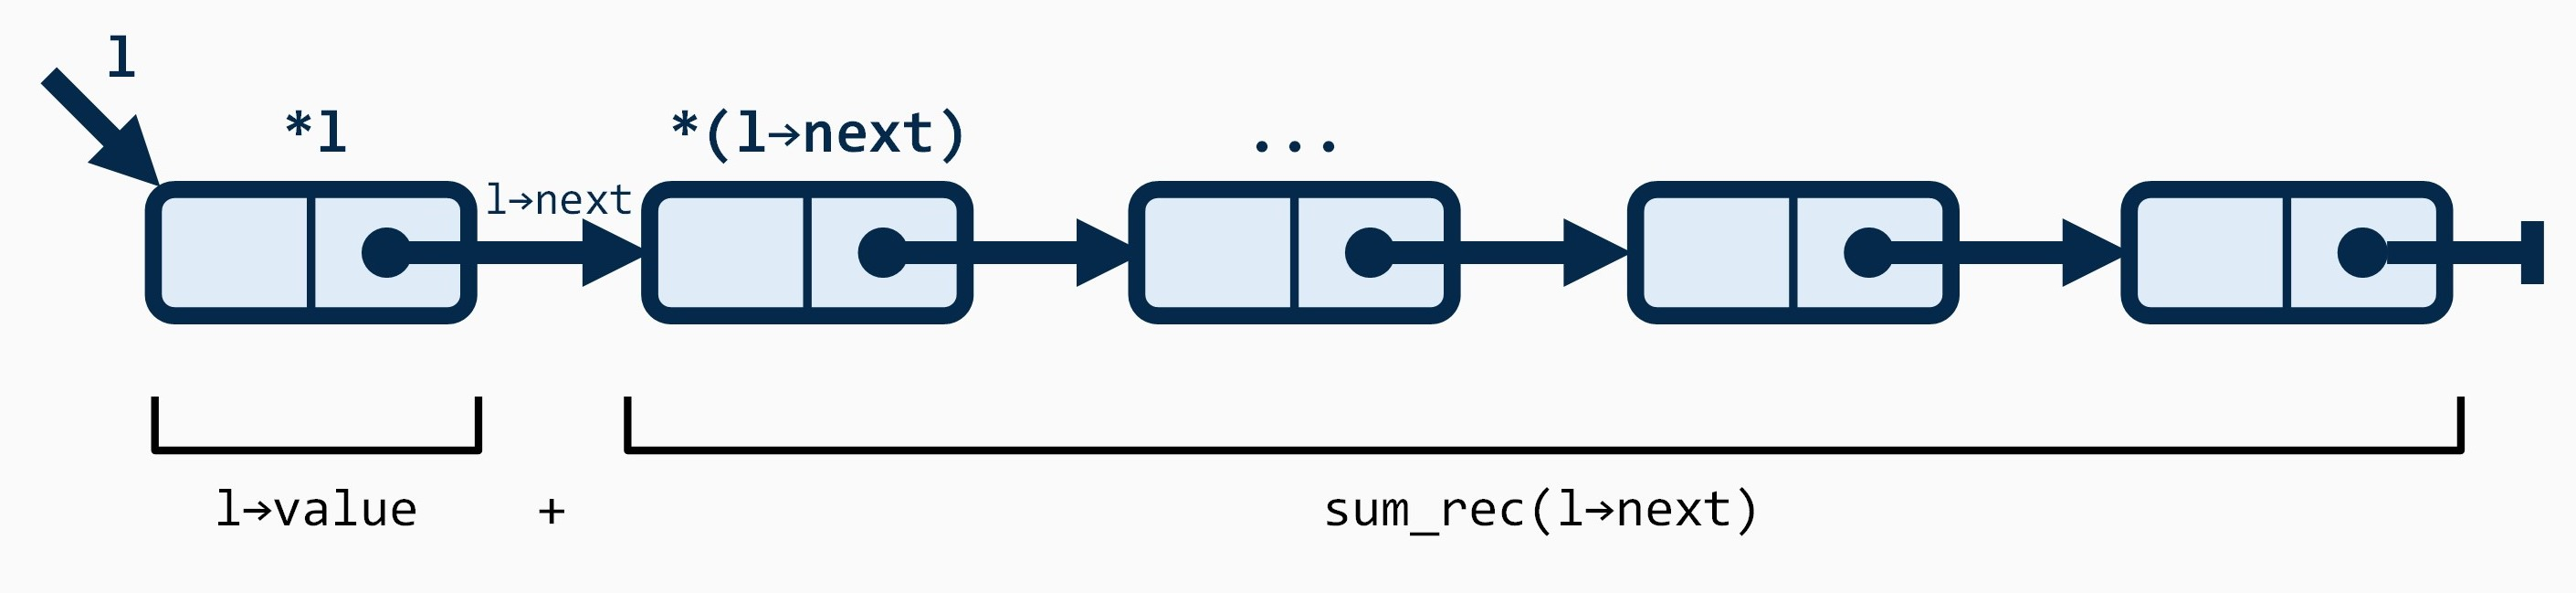
\includegraphics[width=0.8\linewidth]{tut06-graphics/tut06-summe-rec}
	\end{center}

	\pause
		
	\begin{lstlisting}[style=notebook]
	int sum_rec(list l) {
		if (l == NULL) return 0; 
			/* nach letztem element nichts mehr addieren */
		return l->value + sum_rec(l->next); 
			/* nimm key und addiere summe der restliste */
	}
	\end{lstlisting}
\end{frame}

\begin{frame}[fragile] \frametitle{Aufgabe 2 --- Teil (d)}
	\textbf{Löschen von Elementen}
	\begin{center}
		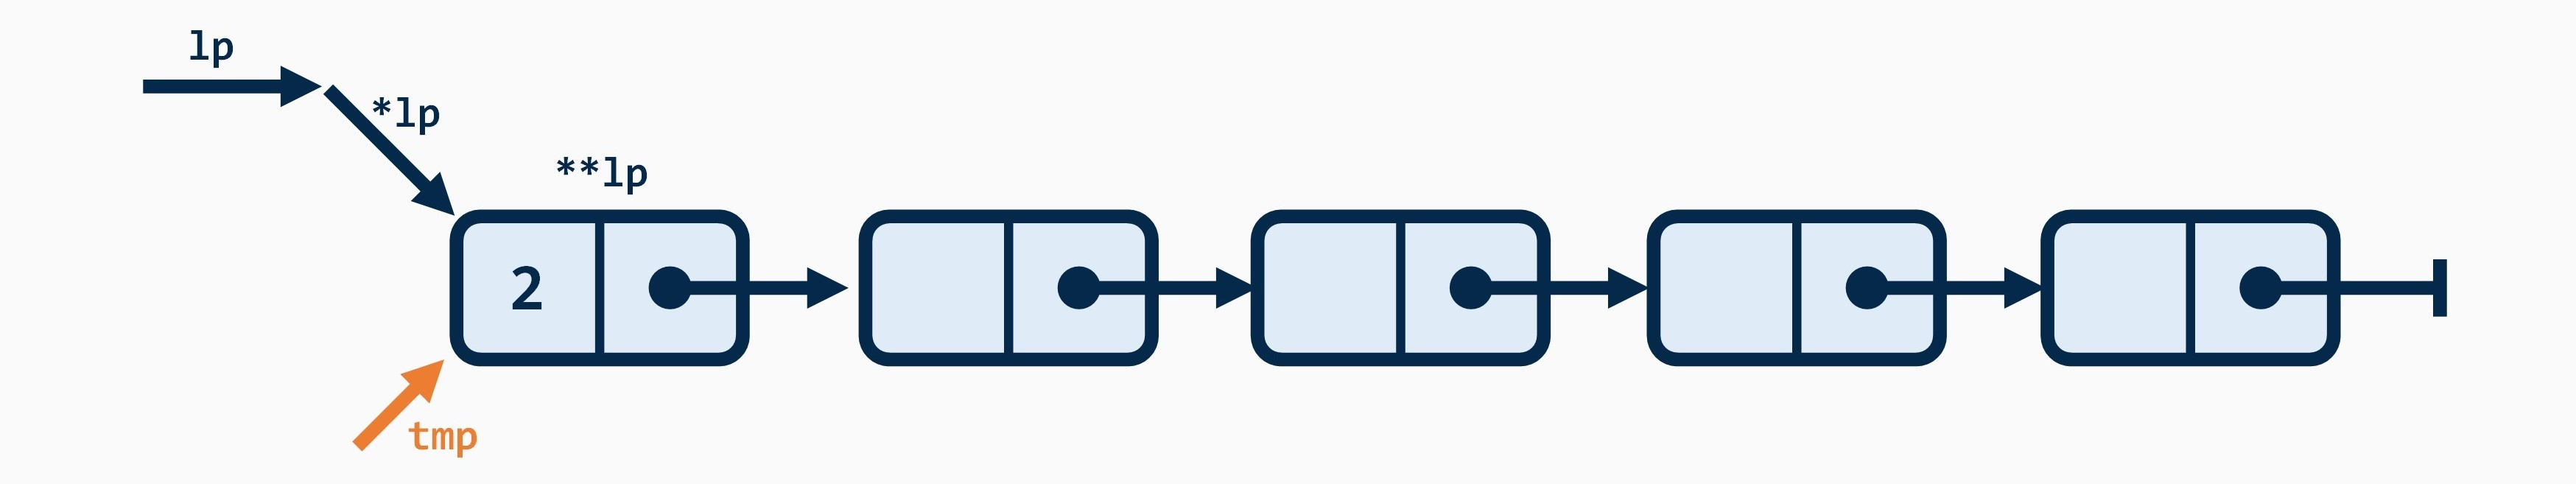
\includegraphics[width=\linewidth]{tut06-graphics/tut06-rmEvans-1} \\ \pause
		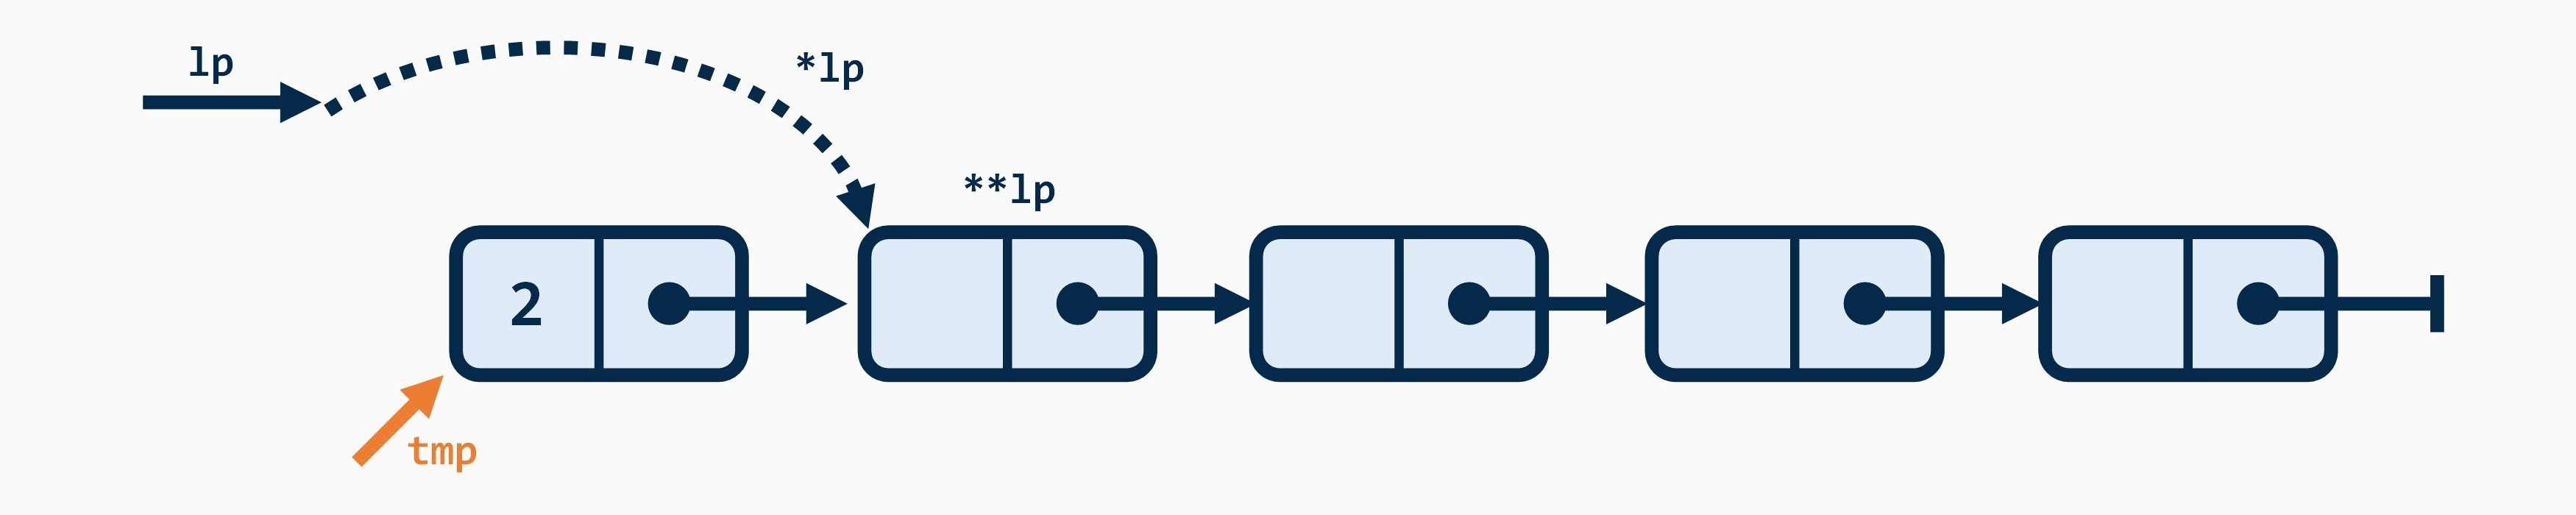
\includegraphics[width=\linewidth]{tut06-graphics/tut06-rmEvans-2} \\ \pause
		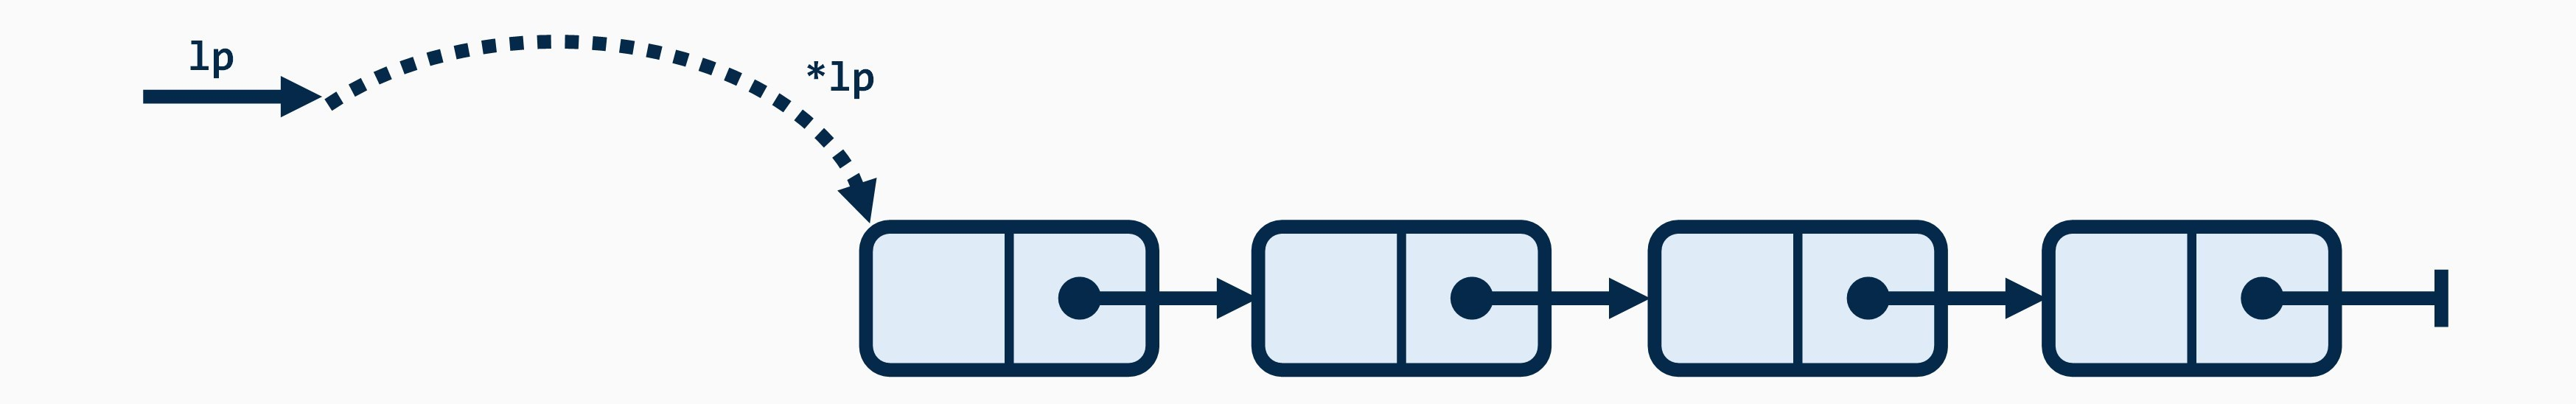
\includegraphics[width=\linewidth]{tut06-graphics/tut06-rmEvans-3}
	\end{center}
\end{frame}


\begin{frame}[fragile] \frametitle{Aufgabe 2 --- Teil (d)}
	\textbf{Löschen von Elementen --- iterativ}
	\begin{itemize}
		\item laufe Liste entlang, solange nicht am Ende angekommen
		\item zeigt \texttt{*lp} auf einen geraden Schlüssel $\to$  \textit{löschen}
		\begin{itemize}
			\item merke Zugriff auf \texttt{*lp} (zu löschen) in \texttt{tmp}
			\item überspringe zu löschendes Element
			\item befreie zu löschendes Element (Zugriff via \texttt{tmp})
		\end{itemize}
	\end{itemize}
	
	\pause
	
	\begin{lstlisting}[style=notebook, basicstyle=\scriptsize\ttfamilywithbold]
	void rmEvens_it(list *lp) {
			while (lp != NULL && *lp != NULL) {
					if ((*lp)->value % 2 == 0) {
							list tmp = *lp;
							*lp = (*lp)->next;
							free(tmp);
					} else
							lp = &(*lp)->next;
			}
	}
	\end{lstlisting}
\end{frame}

\begin{frame}[fragile] \frametitle{Aufgabe 2 --- Teil (d)}
	\textbf{Löschen von Elementen --- rekursiv} \small
	\begin{itemize}
		\item Basisfall: keine Liste oder Liste leer $\to$ tue nichts
		\item Fallunterscheidung bzgl. Schlüsselwert
		\begin{itemize} \footnotesize
			\item gerade: löschen \& Speicher befreien wie in iterativer Variante
			\item ungerade: überspringe dieses Element
		\end{itemize}
		\item verfahre so weiter mit der Restliste
	\end{itemize}
	
	\pause
	
	\begin{lstlisting}[style=notebook, basicstyle=\scriptsize\ttfamilywithbold]
	void rmEvens_rec(list *lp) { 
			if (lp == NULL || *lp == NULL) return ;
			if ((*lp)->value % 2 == 0) {
					list tmp = *lp;
					*lp = (*lp)->next;
					free(tmp);
			} else
					lp = &(*lp)->next;
			rmEvens_rec(lp);  
	}
	\end{lstlisting}
\end{frame}


\begin{frame}[fragile] \frametitle{Aufgabe 2 --- Teil (e)}
	\textbf{neue Liste ohne bestimmte Elemente} \small
	\begin{itemize}
		\item erzeuge neue Liste
		\item laufe durch alte Liste durch -- betrachte Schlüsselwerte
		\begin{itemize} \footnotesize
			\item gerade: Element überspringen
			\item ungerade: an neue Liste anfügen
		\end{itemize}
	\end{itemize}
	
	\pause
	
	\begin{lstlisting}[style=notebook]
	list odds(list lp){
			list erg = NULL; /* erzeuge neue liste */		
			while (lp != NULL ){           
					if (lp->value % 2 != 0) 
							append(&erg, lp->value);
					lp = lp->next;              
			}
			return erg;
	}
	\end{lstlisting}
\end{frame}


%%%%%%%%%%%%%%%%%%%%%%%%%%%%%%%%%%%%%%%%%%%%%%%%%%%%%%%%%%%%%%%%%%%%%%%%%%%%%%%%%%%

\begin{frame}
	\bfseries \centering \Huge
	
	Next Level: 
	
	Bäume
\end{frame}


%%%%%%%%%%%%%%%%%%%%%%%%%%%%%%%%%%%%%%%%%%%%%%%%%%%%%%%%%%%%%%%%%%%%%%%%%%%%%%%%%%%


\end{document}